\ifx\allfiles\undefined
\documentclass[11 pt,t]{beamer}
\geometry{showframe,paperwidth=160mm,paperheight=120mm,margin=5mm,nohead,nofoot,nomarginpar}
%\usetheme[
%bullet=circle,		% Other option: square
%bigpagenumber,		% circled page number on lower right
%topline=true,		% colored bar at the top of the frame 
%]{Zurich}

\usetheme{metropolis}

\usepackage{amsmath}
\usepackage{fontspec,xunicode,xltxtra}
\usepackage{pgf}
\usepackage{tikz}
\usetikzlibrary{patterns}
\usetikzlibrary{plotmarks}
\usetikzlibrary{arrows,decorations.pathmorphing,backgrounds,fit,positioning,shapes,chains}
\definecolor{yellow1}{rgb}{1,0.8,0.2}  
\usepackage{pgfplots}
\pgfplotsset{compat=newest}
\tikzset{elegant/.style={smooth,thick,samples=50,cyan}}
\tikzset{eaxis/.style={->,>=stealth}}

\let\oldequation=\equation
\let\oldendequation=\endequation
\renewenvironment{equation}{\oldequation\textstyle}{\oldendequation}
\setlength{\baselineskip}{0pt}
\renewcommand{\baselinestretch}{0pt}
\setlength{\partopsep}{0pt}
\setlength{\parsep}{0pt}
\setlength{\itemsep}{0cm}
\setlength{\topsep}{0cm}
\setlength{\parskip}{0pt}
\setlength{\lineskip}{0pt}
%\setitemize[1]{itemsep=0pt,partopsep=0pt,parsep=\parskip,topsep=0pt}
%%\usepackage[compatibility=false]{caption}
%%\captionsetup{font={scriptsize}}
\setbeamerfont{caption}{size=\tiny}
\setlength{\abovecaptionskip}{0pt}
\setlength{\belowcaptionskip}{0pt}
\setlength{\abovedisplayshortskip}{0pt}
\setlength{\belowdisplayshortskip}{0pt}
\setlength{\abovedisplayskip}{0pt}
\setlength{\belowdisplayskip}{0pt}
\setlength{\jot}{0pt}
\usepackage{setspace} 
\linespread{1.4}
\fi

\ifx\allfiles\undefined
\begin{document}
\fi
\section{Deep Learning for Image Processing}
% ----------------------------------------------------------------------------
\begin{frame}
\frametitle{Deep Learning for Image Processing: CNN}
	\small
	\begin{itemize}
		\item Convolutional Layer
		\item Pooling Layer
			\\\hspace{1cm} mean-pooling
			\\\hspace{1cm} max-pooling
			\\\hspace{1cm} stochastic-pooling
		\item (Activation Layer)
		\item Full-connected Layer
		\item Network Gallery
			\\\hspace{1cm} LeNet
			\\\hspace{1cm} AlexNet
			\\\hspace{1cm} GoogleLeNet
			\\\hspace{1cm} VGG
			\\\hspace{1cm} ResNet
		\item Feature Extractor \& Fine-tuning
	\end{itemize}
\end{frame}
% ----------------------------------------------------------------------------
\begin{frame}
\frametitle{Convolutional Layer}
	\scriptsize 
	\begin{itemize}
		\item structure
		\\\hspace{0.5cm}	Input is $M$ features $f_{m}^{l-1}$ in previous layer, and out put is $N$ features $f_{n}^l$ in current layer. Convolutional operator between each pair of $f_{m}^{l-1}$ and $f_{n}^{l}$ is a square matrix $\Theta=[\theta_{i,j}]$ filter and a bias $b$. One $f_{m}^{l-1}$ may be corresponding to multiple $f_n^{l}$ and one $f_n^{l}$ may be corresponding to multiple $f_m^{l-1}$. $\Theta$ and $b$ is trainable by
		$\frac{\partial}{\partial{b^l}}=\delta_{f^l}$,
		$\frac{\partial}{\partial{\Theta^l}}=\delta_{f^l}f^{l-1}$.
		\item forward 
		\\\hspace{0.5cm}	Every sub matrix $s$ of feature $k$ in $f_k^{l-1}$ of size $|\Theta|$ is mapped to one element $t$ in $f_{l}$ feature:
		\\\hspace{0.5cm} $t=\sum_{k}Conv(f_k^{l-1},\Theta)=\sum_{k}\sum_{i,j}(S_{i,j}^k\theta_{i,j}^k)$, 
			where matrix coloumn and row are reduced by $|\Theta|^{0.5}-1$, and $k$ is mapping $k$ layer $l-1$ to layer $l$
		\item backward 
		\\\hspace{0.5cm} 1st: padding matrix $\delta_t$ with 0 by $2(|\Theta|^{0.5}-1)$
		\\\hspace{0.5cm} 2nd: rotate $\Theta$ by 180 degree to get $\Theta^{rotate}$ 
		\\\hspace{0.5cm} 3rd: calculate $Conv$ as forward step.
		\\\hspace{0.5cm} In summary,	$\delta_s=\sum_{p}DeConv(\delta_t,\Theta)=\sum_{p}Conv(\delta_t^{padding},\Theta^{rotate})$
		\\\hspace{1cm}where $p$ is mapping layers from $l-1$ to $p$ layers in $l$.
	\end{itemize}
\end{frame}
% ----------------------------------------------------------------------------
\begin{frame}
\frametitle{Convolutional Operation Sample}
	\tiny
	\begin{itemize}
		\item forward $c=Conv(a,b)$
			\begin{equation*}
				a=
				\left\{
					\begin{aligned}
						  &a_1 \ a_2 \ a_3 
						\\&a_4 \ a_5 \ a_6
						\\&a_7 \ a_8 \ a_9
					\end{aligned}
				\right\}
				b=
				\left\{
					\begin{aligned}
						  b_1 \ b_2
						\\b_3 \ b_4 
					\end{aligned}
				\right\}
			\to	c=
				\left\{
					\begin{aligned}
						  c_1=a_1b_1+a_2b_2+a_4b_3+a_5b_4 \qquad c_2=a_2b_1+a_3b_2+a_5b_3+a_6b_4
						\\c_3=a_4b_1+a_5b_2+a_7b_3+a_8b_4 \qquad c_4=a_5b_1+a_6b_2+a_8b_3+a_9b_4
					\end{aligned}
				\right\}
			\end{equation*}
		\item backward $\delta_a=DeConv(\delta_c,b) \qquad $ deduced by $\delta_a=\frac{dy}{da}=\frac{dy}{dc}\frac{dc}{da}=\delta_c\frac{dc}{da}$
			\begin{equation*}
				c=
				\left\{
					\begin{aligned}
						   &0 \ \ \  0 \ \ \ 0 \ \ \ 0
						\\ &0 \  \delta_{c_1} \ \delta_{c_2} \ 0
						\\ &0 \  \delta_{c_3} \ \delta_{c_4} \ 0
						\\ &0 \ \ \  0 \ \ \ 0 \ \ \ 0
					\end{aligned}
				\right\}
				b=	
				\left\{
					\begin{aligned}
						  b_4 \ b_3
						\\b_2 \ b_1 
					\end{aligned}
				\right\}
		\to	
				a=
				\left\{
					\begin{aligned}
						  &\delta_{a_1}
						  \delta_{a_2}
						  \delta_{a_3}
					   \\ &\delta_{a_4}
						  \delta_{a_5}
						  \delta_{a_6}
					   \\ &\delta_{a_7}
						  \delta_{a_8}
						  \delta_{a_9}
					\end{aligned}
				\right\}
			\end{equation*}
			\begin{equation*}
					\begin{aligned}
						  &\delta_{a_1}=\delta_{c_1}b_1  
						  &&\delta_{a_2}=\delta_{c_1}b_2+\delta_{c_2}b_1 
						  &&\delta_{a_3}=\delta_{c_2}b_2  
					   \\ &\delta_{a_4}=\delta_{c_1}b_3+\delta_{c_3}b_1 
						  &&\delta_{a_5}=\delta_{c_1}b_4+\delta_{c_2}b_3+\delta_{c_4}b_1 
						  &&\delta_{a_6}=\delta_{c_2}b_4+\delta_{c_4}b_2 
					   \\ &\delta_{a_7}=\delta_{c_3}b_3
						  &&\delta_{a_8}=\delta_{c_3}b_4+\delta_{c_4}b_3
						  &&\delta_{a_9}=\delta_{c_4}b_4
					\end{aligned}
			\end{equation*}
	\end{itemize}
\end{frame}
% ----------------------------------------------------------------------------
\begin{frame}
\frametitle{Pooling Layer}
	\scriptsize
	\begin{itemize}
		\item structure
			\\Generally, pooling operator is a square matrix of size $2*2$, but is not absolute. If there is one feature mapping between layer $l-1$ and layer $l$, there is a pooling operator. It is not trainable generally, but sometimes there is trained weighted inside pooling operator.
		\item forward: Every sub matrix $s$ of a feature $f_{l-1}$ is mapped to one element $t$ in $f_{l}$ feature:
			\\\hspace{0.5cm} Max Pooling:$t=Pooling_{max}(s)=max_i(s_i)$
			\\\hspace{0.5cm} Average Pooling:$t=Pooling_{average}(s)=\frac{\sum_i(s_i)}{4}$
			\\\hspace{0.5cm} Stochastic Pooling:$t=Pooling_{stochastic}(s)=multinomial\frac{s_i}{\sum_i(s_i)}$
		\item backward: Padding one element in $\delta_l$ to $2*2$ element in $\delta_{l-1}$.
			\\\hspace{0.5cm} Max Pooling: filling the element which is max in forward with $\delta_l$, and three others with 0.
			\\\hspace{0.5cm} Average Pooling: filling all 4 elements of $\delta_{l-1}$ with $\delta_l/4$.
			\\\hspace{0.5cm} Stochastic Pooling: filling the chosen element in foward of $\delta_{l-1}$ with $\delta_l$, and three others with 0.
	\end{itemize}
\end{frame}
% ----------------------------------------------------------------------------
\begin{frame}
\frametitle{Pool Operation Sample}
	\tiny
	\begin{itemize}
		\item forward $c=Pooling_{max}(a)$
			\begin{equation*}
				a=
				\left\{
					\begin{aligned}
						  &a_1 \ a_2 \ a_3 \ a_4
						\\&a_5 \ a_6 \ a_7 \ a_8
						\\&a_9 \ a_{10} \ a_{11} \ a_{12}
						\\&a_{13} \ a_{14} \ a_{15} \ a_{16}
					\end{aligned}
				\right\}
			\to	c=
				\left\{
					\begin{aligned}
						  &c_1=a_2=max\{a_1,a_2,a_5,a_6\} \qquad c_2=a_7=max\{a_3,a_4,a_7,a_8\}
						\\  &c_3=a_9=max\{a_9,a_{10},a_{13},a_{14}\} \qquad c_4=a_{16}=max\{a_{11},a_{12},a_{15},a_{16}\}
					\end{aligned}
				\right\}
			\end{equation*}
		\item backward $\delta_a=DePooling(\delta_c) \qquad $ deduced by $\delta_a=\frac{dy}{da}=\frac{dy}{dc}\frac{dc}{da}=\delta_c\frac{dc}{da}$
			\begin{equation*}
				c=
				\left\{
					\begin{aligned}
						 \delta_{c_1} \ \delta_{c_2} 
						\\ \delta_{c_3} \ \delta_{c_4}
					\end{aligned}
				\right\}
		\to	
				a=
				\left\{
					\begin{aligned}
						  &0 \quad \delta_{c_1}  0 \quad  0
						\\  &0 \quad 0 \quad  \delta_{c_2}  0
						\\  & \delta_{c_3}  0   \quad 0 \quad  0
						\\  &0 \quad 0 \quad  0 \quad  \delta_{c_4} 
					\end{aligned}
				\right\}
			\end{equation*}
	\end{itemize}
\end{frame}
% ----------------------------------------------------------------------------
\begin{frame}
\frametitle{Activation Layer}
	\small
	\begin{itemize}
		\item structure
			\\Generally, activation layer $l$ is of the same size as previous layer $l-1$. It maps from pixel $s_i^{l-1}$ to pixel $t_i^{l}$ by nonlinear function $f$. In addition, there is trainable parameter $\Theta$ and $b$ for input pixel. Its previous layer may be convolutional or pooling layer.
		\item forward: pixel $s_i^{l-1}$ to pixel $t_i^{l}$ mapping is formulated as:
			\\\hspace{0.5cm} $t_i^{l}=f(\Theta s_i^{l-1}+b)$
		\item backward: Trivally as:
			\\\hspace{0.5cm} $\delta_i^{l-1}=\delta_i^l f^{\prime} \Theta$
	\end{itemize}
\end{frame}
% ----------------------------------------------------------------------------
\begin{frame}
\frametitle{LeNet-5}
	\small
	\begin{itemize}
		\item Architecture
			\centerline{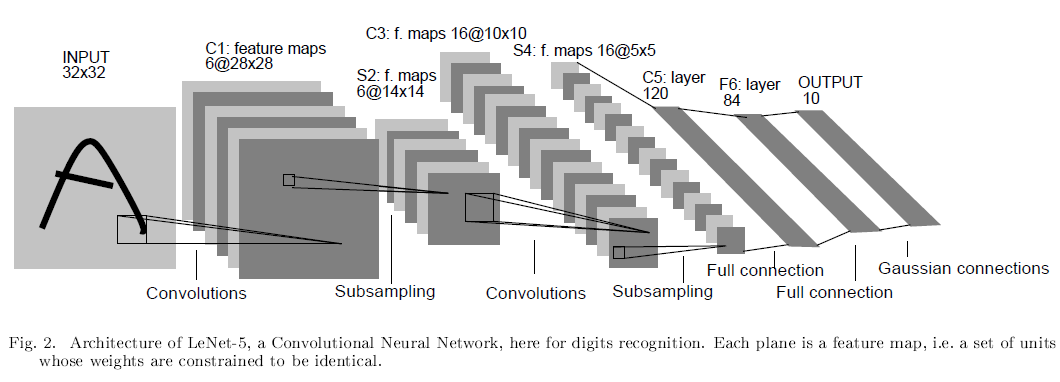
\includegraphics[height=3.5cm]{LeNet-5.png}}
	\end{itemize}
\end{frame}
% ----------------------------------------------------------------------------
\begin{frame}
\frametitle{LeNet-5}
	\small
	\begin{itemize}
		\item domain: hand-writing number recognition
		\item structure:
		\\\hspace{0.5cm}input: 32*32
		\\\hspace{0.5cm}C1: by 6 Conv 5*5, 6*28*28
		\\\hspace{0.5cm}S2: by Weighted Mean Pool 2*2, 6*14*14
		\\\hspace{0.5cm}C3: by 6 Conv 5*5, 16*10*10
		\\(0,1,2)->0
		(1,2,3)->1
		(2,3,4)->2
		(3,4,5)->3
		(4,5,0)->4
		(5,0,1)->5
		(0,1,2,3)->6
		(1,2,3,4)->7
		(2,3,4,5)->8
		(3,4,5,0)->9
		(4,5,0,1)->10
		(5,0,1,2)->11
		(0,1,3,4)->12
		(1,2,4,5)->13
		(0,2,3,5)->14
		(0,1,2,3,4,5)->15
		\\\hspace{0.5cm}S4: by Weighted Mean Pool 2*2, 16*5*5
		\\\hspace{0.5cm}C5: by 16 Conv 5*5, 120*1*1
		\\\hspace{0.5cm}F6: by full connected, 84*1*1
		\\\hspace{0.5cm}Output: by full connected, 10*1*1
	\end{itemize}
\end{frame}
% ----------------------------------------------------------------------------
\begin{frame}
\frametitle{AlexNet}
	\small
	\begin{itemize}
		\item Architecture
			\centerline{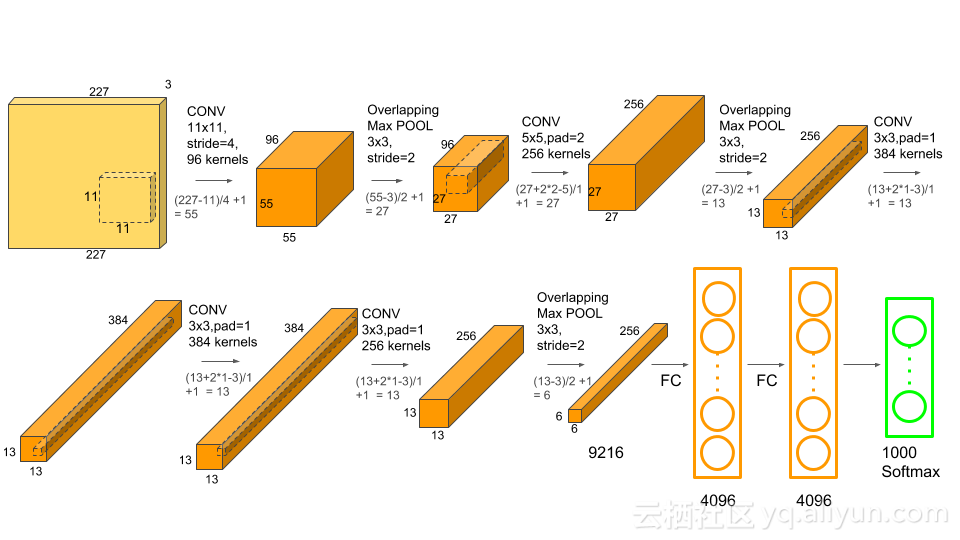
\includegraphics[height=3.5cm]{AlexNet.png}}
			%\centerline{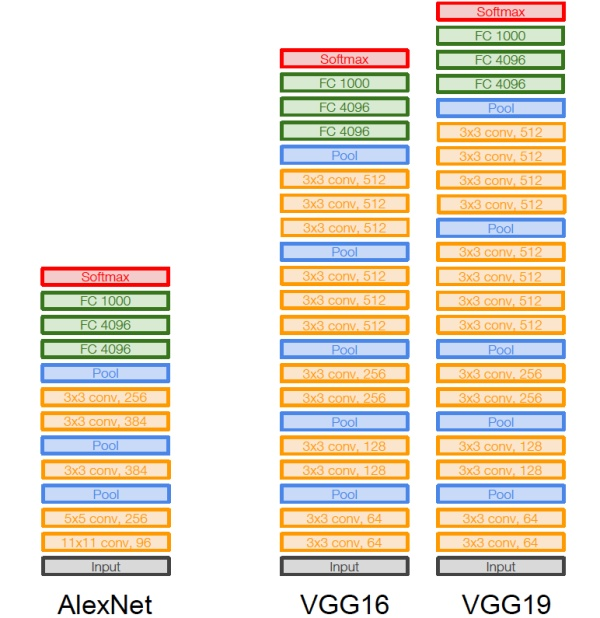
\includegraphics[height=3.5cm]{AlexNet-detail.jpg}}
	\end{itemize}
\end{frame}
% ----------------------------------------------------------------------------
\begin{frame}
\frametitle{VGG}
	\small
	\begin{itemize}
		\item Architecture
			\centerline{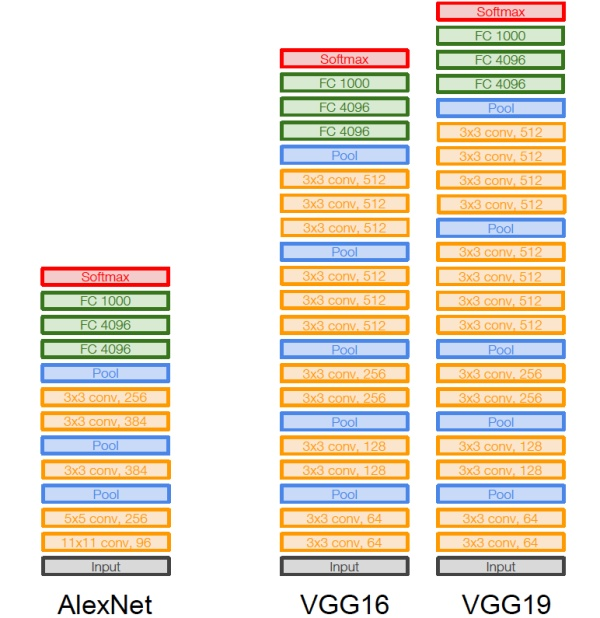
\includegraphics[height=7cm]{AlexNet-detail.jpg}}
	\end{itemize}
\end{frame}
% ----------------------------------------------------------------------------
\begin{frame}
\frametitle{GoogLeNet}
	\small
	\begin{itemize}
		\item Architecture
			\centerline{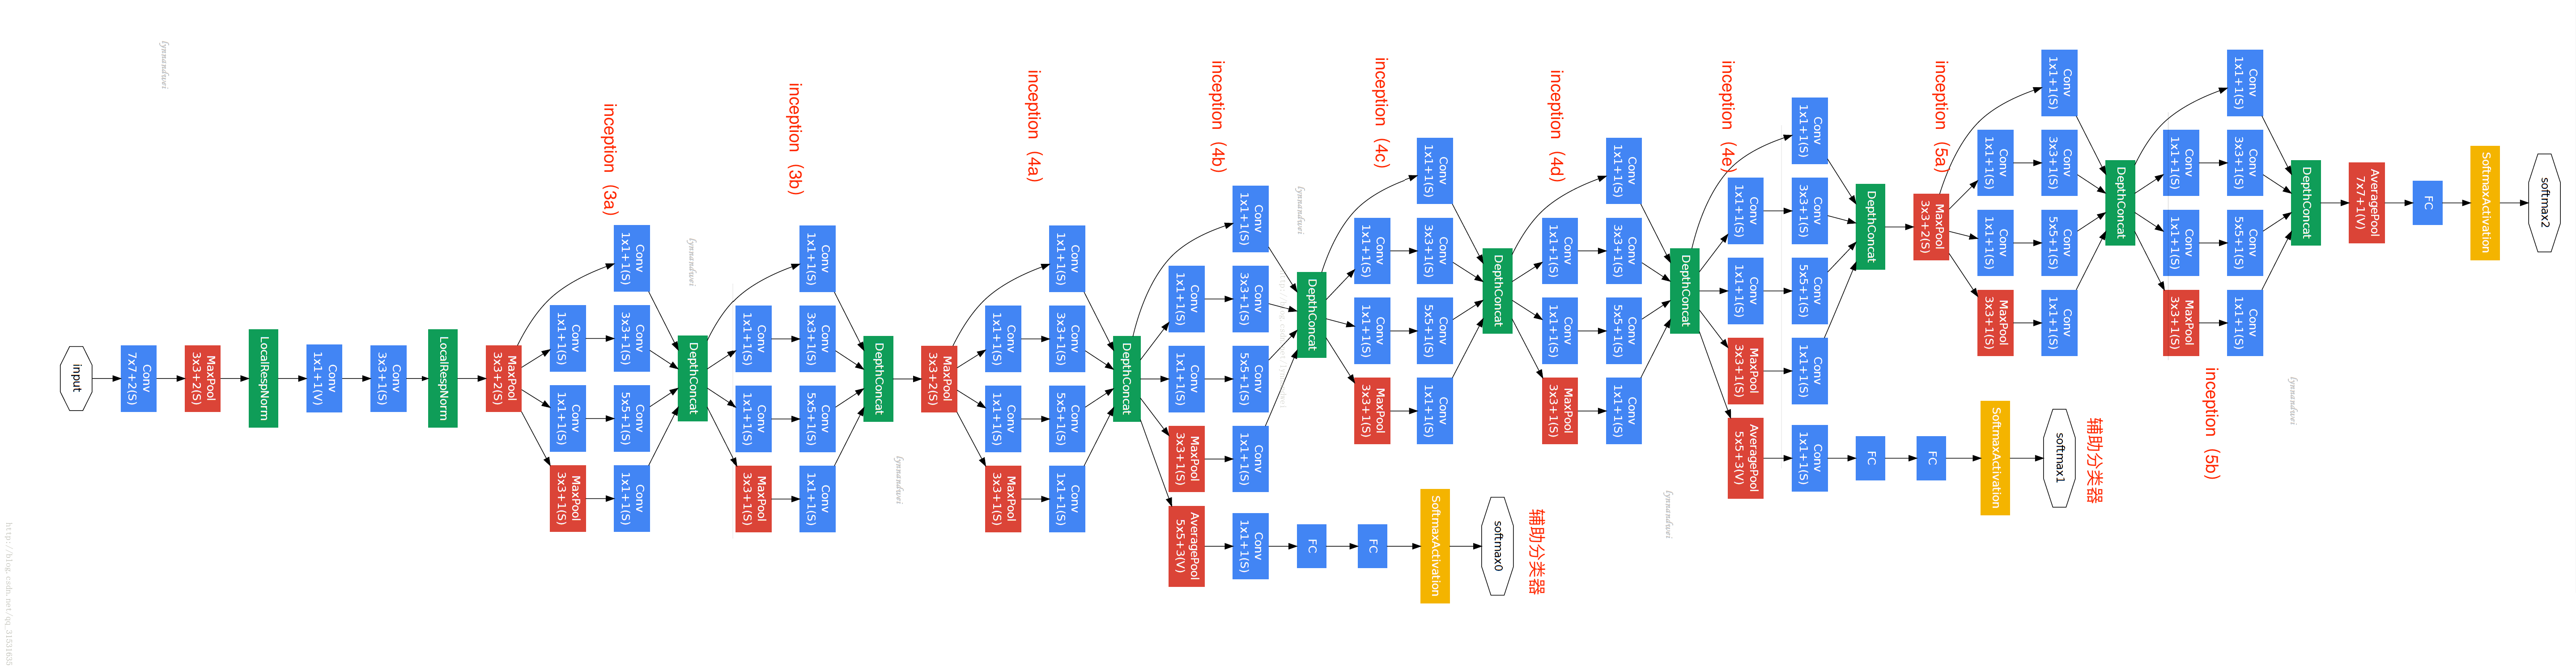
\includegraphics[height=6cm]{GoogLeNet.png}}
	\end{itemize}
\end{frame}
% ----------------------------------------------------------------------------
\begin{frame}
\frametitle{ResNet}
	\small
	\begin{itemize}
		\item Architecture
			\centerline{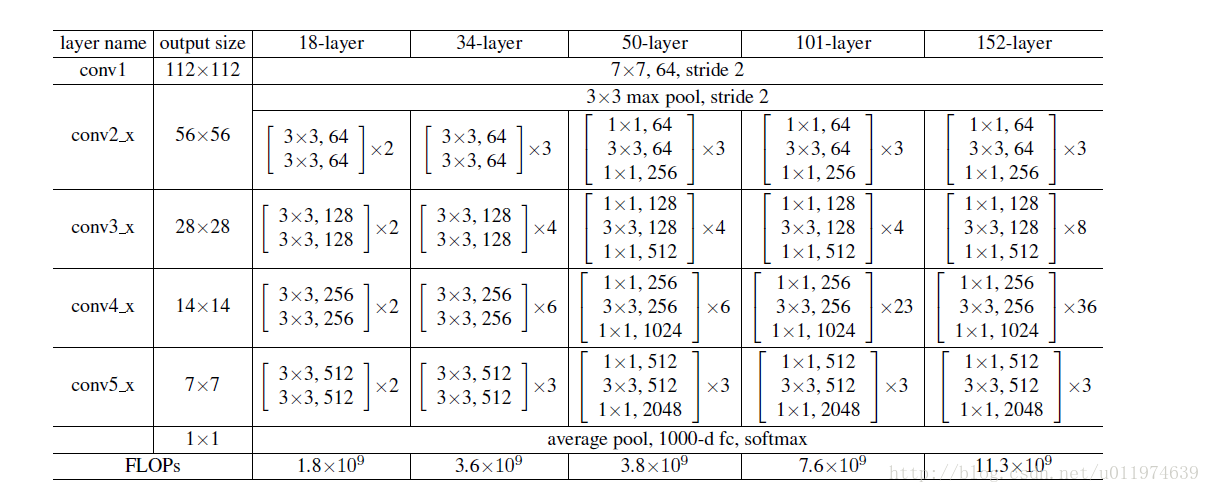
\includegraphics[height=5cm]{ResNet.png}}
	\end{itemize}
\end{frame}
% ----------------------------------------------------------------------------
\ifx\allfiles\undefined
\end{document}
\fi
